
\chapter{CALock: Multi-Granularity locking and conflict detection} \label{chap:calock}

\minitoc

In Chapter \ref{chap:theory}, we discussed the theory behind CALock labelling. We introduced \lstinline|BFLabel()|, a function used to preprocess a hierarchy. Once preprocessed, each vertex in a hierarchy is assigned a unique label. These labels are used to identify a grain for a lock request for a set of lock targets. 


Recall from Chapter \ref{chap:background}, a standard MGL lock protocol involves the following steps:

\begin{enumerate}
	\item Optional preprocessing
	\item Preparing a lock request \label{step:prep}
	\item Requesting a lock
	\item Performing an operation
	\item Optional metadata maintenance
	\item Releasing the lock \label{step:release}
\end{enumerate}

In this chapter, we will study steps \ref{step:prep}-\ref{step:release} in detail for CALock. We will introduce the lock request schema for CALock as well as a lock pool which is used to detect conflicts between requests. We will discuss how we avoid typical \emph{time of check to time of use} (TOCTOU) race conditions between threads and specific optimizations made to the lock pool for fairness.

% In Chapter \ref{chap:theory}, we discussed the formal theory behind CALock. A recursive function \inline|BFLabel()| was introduced to assign labels to the vertices in the graph. These labels are used to identify the lock grain of a lock request. Labelling is performed as an initialization step and is not required during runtime. Once a hierarchy is labelled, threads can utilize the labels to lock the graph at different granularities. From the locking steps discussed in Chapter \ref{chap:background}, Section \ref{sec:lockAcquisitionProtocol}, we know that a thread wishing to lock a set of vertices must first create a lock request and then check for conflicts with other lock requests. Once the lock request is granted, a thread can proceed to its critical section, following which, it releases the lock.

% In CALock, a lock request contains information derived from the labels of the vertices in the lock request which is used to identify the lock guard. Lock requests are added to a concurrent data structure called a lock pool. This pool is used to detect conflicts between lock requests. After adding a lock request to the pool, a thread checks for conflicts with other lock requests in the pool. If no conflict is detected, the thread proceeds to its critical section. This process is shown in Listing \ref{lockFunction}. The main steps are: 

% \begin{enumerate}
% 	\item \textbf{Lock grain identification}: A thread uses the labels of the vertices in its lock request to identify the grain it wants to lock. The thread then determines the lock guard associated with this grain and locks it.
% 	\item \textbf{Lock request creation}: The thread proceeds to create a lock request for the guard and adds it to a lock pool. 
% 	\item \textbf{Lock conflict detection}: After adding its request, the thread evaluates potential conflicts by comparing its request with other entries in the pool. In CALock, two conditions indicate a lock conflict. If both conditions hold for a pair of lock requests, they are in conflict.
% 	\item \textbf{Operation execution}: If no conflict is detected, the thread proceeds to execute its operation.
% 	\item \textbf{Lock release}: After the operation is complete, the thread releases the lock on the grain.
% \end{enumerate}

% In this chapter, we look at each of these steps in detail with examples and corner cases. We also discuss the implementation of CALock 
% First, a thread identifies the grain it wishes to lock by using the labels of the vertices in its lock request. This grain is guarded by a lock guard which is to be locked by the thread. 

% Then, the thread proceeds to create a lock request for the guard and adds it to a lock pool. 

% Finally, the thread checks for conflicts with other lock requests in the pool and blocks if a conflict is detected.

\section{Lock request preparation: Vertex labels and LGCA}

After a hierarchy is preprocessed, threads start accessing data on vertices. This data access is a read or a write operation. Often, threads wish to access multiple data items atomically. Once the set of vertices (lock targets) to be accessed  is identified, the thread accessing them needs to ensure isolation to guarantee correctness. To achieve this, it requests a lock on the \emph{Lowest Guarding Common Ancestor} (LGCA) of the set of lock targets. With CALock, this is done by taking the set intersection of the labels of the lock targets. It follows from Theorem \ref{proofOfDeepness} that the last element in this set intersection is the LGCA of the set of lock targets and is the root of the grain that contains the target vertices. 

For example, in Figure \ref{calockexample}, Let us lock target vertices H and J. The intersection of their labels is $\{A, C, H\} \cap \{A, C, G, J\} =  \{A,C\}$ in which is C is the deepest vertex. The thread then proceeds to acquire a lock on C. 



% \section{Lock grain identification}
% The lock grain of a set of target vertices in CALock is the smallest sub-graph that contains all the targets, such that all paths to these targets can be guarded against concurrent conflicting access. The guard corresponding to a lock request is the \emph{Lowest Guarding Common Ancestor} (LGCA) of the targets. As shown by Theorem \ref{proofOfDeepness}, the LGCA is the deepest vertex in the graph that is an ancestor of all the lock targets. It is present on all the paths that lead to the vertices to be locked and guards them. 

% In order to lock a set of vertices, the approach in CALock is to find the smallest subgraph that contains all the vertices to be locked such that all the paths to these vertices an be guarded to avoid race conditions. This achieved by finding the \emph{Lowest Guarding Common Ancestor} (LGCA) of the vertices to be locked. As shown in Theorem \ref{proofOfDeepness}, the LGCA is the deepest vertex in the graph that is an ancestor of all the lock targets. It is present on all the paths that lead to the vertices to be locked and guards them, serving as a lock \emph{guard}.

\begin{figure}[h]
	\centering
	\captionsetup{justification=centering}
	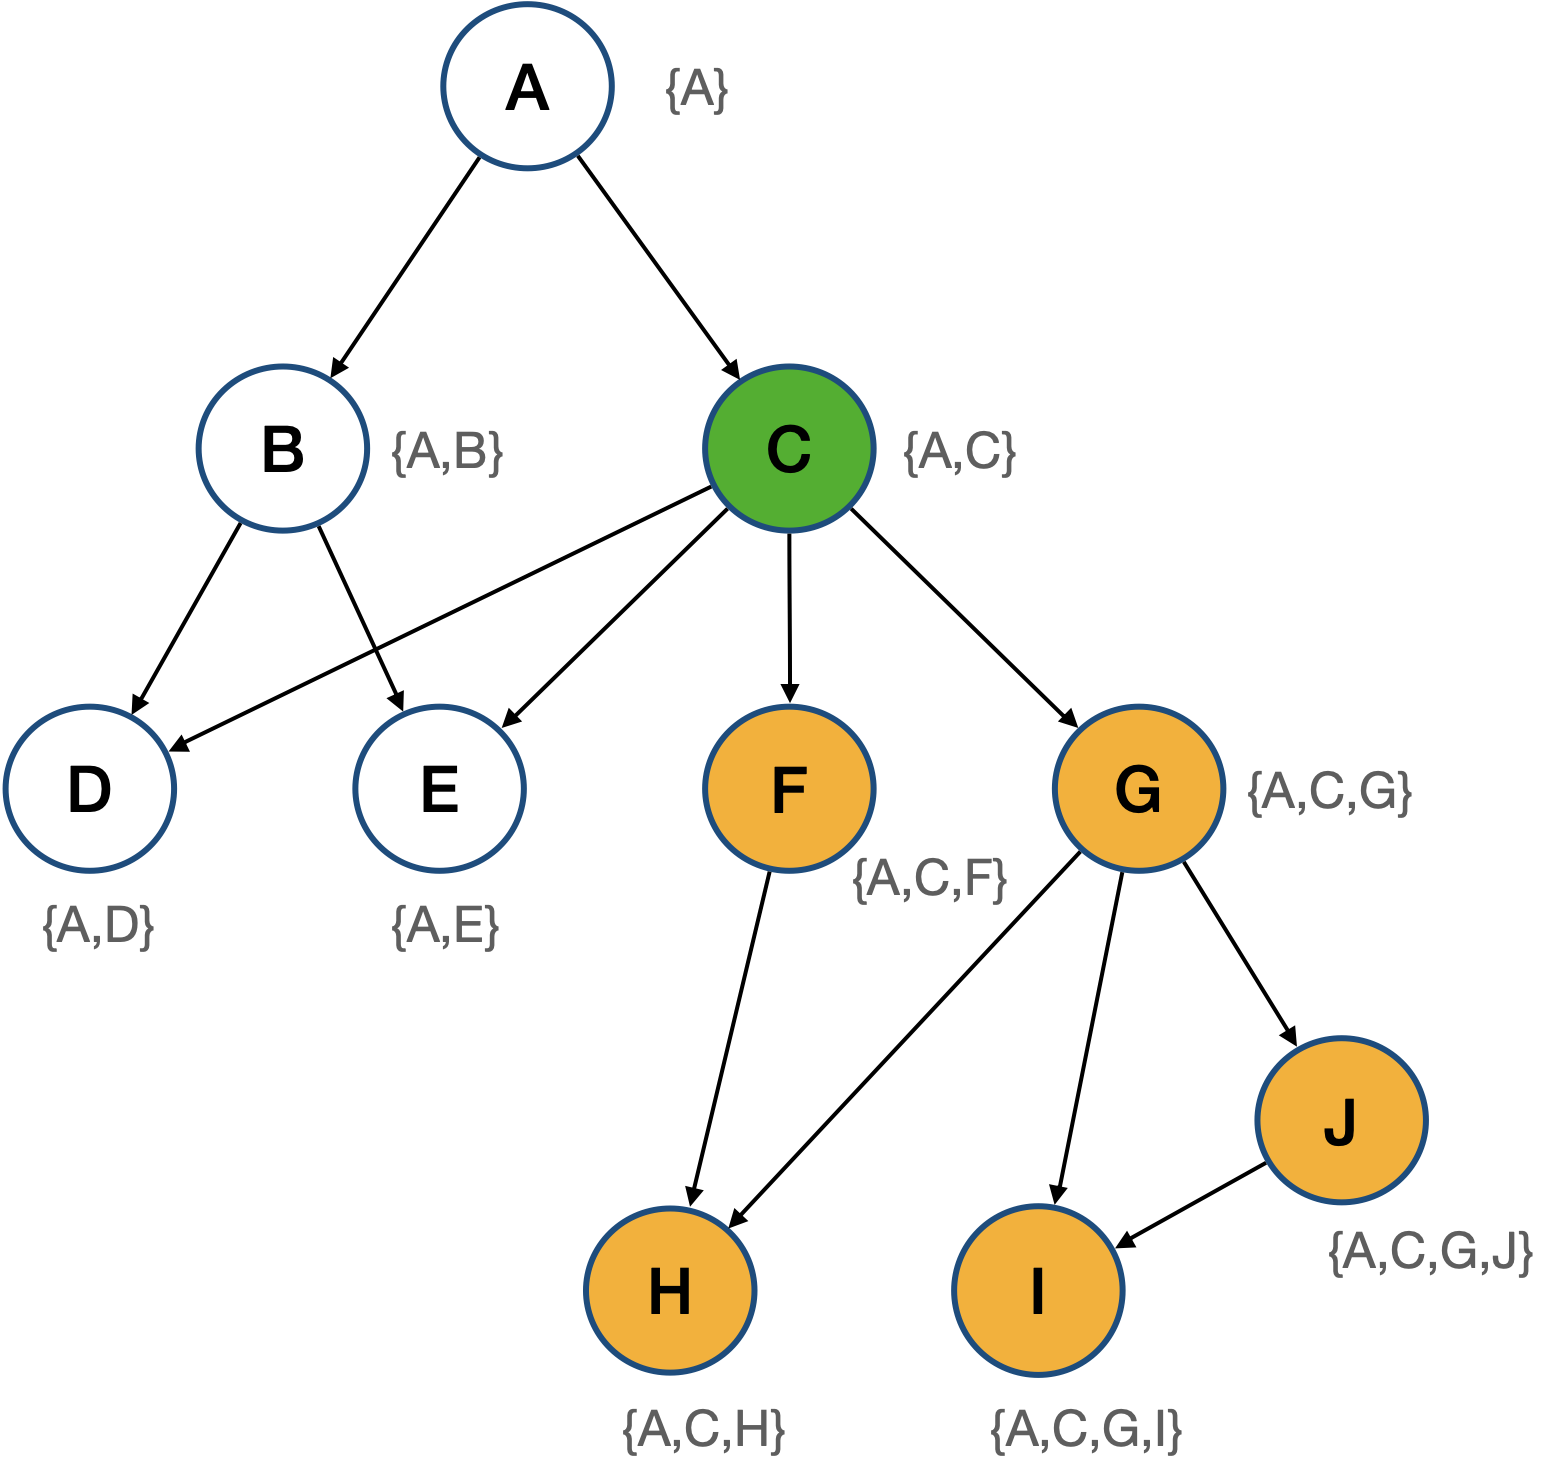
\includegraphics[width=.6\columnwidth]{figures/CALockExample_locked.png}\\
	{\small
		Lock on C: \{A,C\} with grain: \{F, G, H, I, J\}
	}
	\caption{CALock labels}
	\label{calockexample}
\end{figure}

A lock request is created which contains data that identifies its grain without the need to traverse the graph. The lock request contains the following information.

\begin{itemize}
	\item \textbf{Thread ID}: The unique identifier of the thread making the lock request. This helps distinguish lock requests originating from different threads in the system.
	\item \textbf{Guard ID}:The unique identifier of the lock guard, which corresponds to the vertex being locked to control access to a specific portion of the hierarchical data.
	\item \textbf{Guard label}: The label of the lock guard vertex.
	\item \textbf{Sequence number}: A unique number assigned by the lock manager to the lock request when it is added to the lock pool. This sequence number helps in ordering lock requests and ensuring fairness in lock acquisition.
	\item \textbf{Activity Indicator}: A flag or marker used by other threads to monitor the status of this lock request. When a conflict occurs, threads use this indicator to determine whether they need to wait for the current lock request to complete.
	\item \textbf{Lock mode}: Specifies the type of access the thread is requesting for the resource. This can be either read (shared access, allowing concurrent reads) or write (exclusive access, preventing other reads or writes).
\end{itemize}

Each thread creates a lock request for every lock it wishes to acquire. At any given time, a thread can only issue a single lock request, which might contain multiple targets. These lock requests are then added to a pool which begins the procedure of lock acquisition. 

% These fields will be used to detect conflicts with other lock requests. 
% As soon as the thread identifies the LGCA, it issues a lock request by adding its request to a pool used to identify conflicts. 

% \begin{lstlisting}
% class lockObject {
% 	set<char> *criticalAncestors;
% 	int Id;
% 	int mode;
% 	long Oseq;
% 	atomic_flag accessController = ATOMIC_FLAG_INIT;
% }
% \end{lstlisting}

\section{Requesting a lock: Lock pool and lock conflicts}
Once a thread has created a lock request, it calls the \lstinline|LOCK()| function to add the lock request to a pool, indicating an active lock request which can be tested for conflicts with other threads. The procedure for acquiring a lock is shown in Listing \ref{lockFunction}

\subsection{Lock Pool}
The lock pool in CALock is a central data structure used to manage and coordinate lock requests from multiple threads. It is an array where each entry corresponds to a thread and an entry in the lock pool at a thread's index indicates an active lock request from that thread.

The first step taken by the scheduler is to assign a sequence number to the lock request (line \ref{seqNoAllocation}). Sequence numbers help in ensuring fairness by granting locks in a first-come first-served order. Then, the activity indicator for a request is set to true and finally, it is added to the pool at the requesting thread's index. 


% When a thread requests a lock, it is assigned a sequence number and sets its activity indicator to true, signaling that it is actively using the lock. The lock pool helps detect conflicts between lock requests, and CALock uses the sequence numbers to ensure fairness by granting locks in a first-come, first-served manner. Threads check for conflicts and, if necessary, block until the active thread releases the lock, maintaining synchronization and preventing thread starvation.

% The procedure of acquiring a lock is specified in listing \ref{lockfunction}. Initially and when the thread is not holding a lock, its entry is \inline|NULL|. When a thread arrives in the lock pool, it is given a sequence number (line \ref{seqNoAllocation}) and it sets its activity indicator to true (line \ref{waitTrue}) indicating that it is active and using the lock. In order to remain fair and prevent thread starvation, CALock uses sequence numbers to resolve conflicts. The \emph{sequence numbers} are an indication of the order in which the locks are requested. In the presence of conflicts, threads are granted locks in a \emph{first come first serve} order. Other threads check for conflicts with this thread and block until the activity indicator is set to false.

An example of a lock pool containing 3 requests from threads $T_1$, $T_2$ and $T_7$ is shown in Figure \ref{fig:lockPool}. 

\begin{table}[H]
	\centering
	\captionsetup{justification=centering}
	\begin{tabular}{cccccc}
		\textbf{Thread ID} & \textbf{Guard ID}& \textbf{Guard Label} & \textbf{Seq. No.} & \textbf{Active} & \textbf{Mode} \\
		\hline
		$1$ & G &\{A,C,G\} & 2 & true & read\\
		$2$ & C &\{A,C\} & 3   & true & write\\
		$7$ & B &\{A,B\} &  1  & true & read\\
	\end{tabular}
	\caption{Lock requests in the lock pool}
	\label{lockPoolTable}
\end{table}
% \begin{itemize}
% 	\item \{\texttt{TID:1, GuardID:G, GuardLabel:\{A,C,G\}, SeqNo.:2, Active:true, Mode:read}\}
% 	\item \{\texttt{TID:2}\}
% \end{itemize}



Guaranteeing FCFS order for granting locks is essential to ensure fairness. However, a race condition might occur between two concurrent threads where a thread with a higher sequence number and conflicting request is granted a lock before a thread with a lower sequence number could add its request to the pool. 

For example, consider two threads, $T_1$ and $T_2$, both requesting a write lock on the same vertex $v$. Obviously, $T_1$ and $T_2$ cannot be granted their locks in parallel. One of these threads has to wait. $T_1$ is given sequence number 1 and $T_2$, which arrives after, is given sequence number 2. However, $T_1$ is preempted before it can insert its request into the pool and $T_2$ adds its request first, tests for conflict and finds that there is no conflicting request in the pool. Then $T_1$ resumes and inserts its entry into the lock pool. 
At this point, both $T_1$ and $T_2$ will be granted their requests even though they are conflicting. Vertex $v$ is not isolated anymore. This is because, $T_2$ tested for a conflict while $T_1$ had not added its request to the pool and $T_1$ assumes priority since it arrived first and has a sequence number 1.

To avoid this race, the assignment of a sequence number and the addition of the request to the pool is done atomically. We achieve this, in our implementation, with a mutex over the lock pool. Since these two operations are short, serializing threads over with a mutex does not hinder performance. 

% The order in which threads arrive is important to ensure fairness. To prevent a race condition where a thread with a higher sequence number and conflicting request is granted a lock before a thread with a lower sequence number could add its request to the pool, the assignment of a sequence number and the addition of the lock request to the pool is done atomically. 
Once a lock request is added to the pool, it is guaranteed to be granted in FCFS order. After adding its request to the pool, a thread proceeds to check for conflicts with other requests in the pool.


% This is because the thread checks for conflicts with other requests in the pool from left to right. If a conflict is detected, the thread blocks and waits for the conflicting thread to release the lock. Once the lock is released, the thread proceeds to check for conflicts with the remaining threads in the pool. This process is repeated until the thread reaches the end of the lock pool. At this point, the thread is guaranteed to either have no conflicts or have priority over all conflicts because of its sequence number. We discuss this more in Chapter \ref{chap:formalProperties}.

\subsection{Lock conflicts}


% \section{Identifying lock conflicts} \label{lockPool}

In MGL on graphs, conflict detection involves checking two conditions to ensure correctness. These conditions arise from the existence of locks at different granularities (sub-graphs). The compatibility matrix for CALock is shown in Table \ref{compatibilityMatrix}
\begin{itemize}
	\item \textbf{Grain Overlap}: A grain overlap conflict occurs when a writer attempts to acquire a lock at a finer granularity (e.g., a vertex or edge) while another thread holds a lock at a coarser granularity (e.g., a sub-graph or the entire graph). In this case, the finer-grained lock must be exclusive, meaning no conflicting lock can exist at a higher level. For example, if a writer locks a vertex, no lock can be acquired in the grain rooted at that vertex. 
	
	Grain overlaps are checked using the guard ID and guard label of the requests. For two lock requests $R_1$ and $R_2$, if the guard ID of $R1$ is present in the guard label of $R_2$ or vice-versa, then the grains overlap.
	
	\item \textbf{Mode Conflict}: A mode conflict occurs when the grains protected by two lock guards overlap in such a way that a writer’s lock would violate exclusivity. Specifically, if a writer attempts to lock a vertex or edge, and another lock already protects a grain containing said vertex/edge that overlaps with the writer’s lock, the two locks cannot coexist.
	
	Mode conflict is checked by comparing the lock modes for requests in the lock pool. If one request is a write lock and the other is a read lock, then a mode conflict exists.
\end{itemize}



\begin{table}[h]
	\centering
    \captionsetup{justification=centering}
	\begin{minipage}{0.6\textwidth}
		\centering
		\begin{tabular}{c|cc}
			&$rl_i(x)$   &$wl_i(x)$\\
			\hline
			\rowcolor{gray!20}
			$rl_j(y)$& \ding{51} & \ding{68}\\
			$wl_j(y)$& \ding{68}&\ding{68}\\
		\end{tabular}
	\end{minipage}
	\begin{minipage}{0.19\textwidth}
		\begin{flushleft}
			\begin{tabular}{l}
				\scriptsize
				\ding{51} compatible. \\
				% \ding{55} incompatible.\\
				\scriptsize
				\ding{68} compatible iff grain of x \\ \quad \scriptsize is disjoint from grain of y.
			\end{tabular}
		\end{flushleft}
	\end{minipage}
	\\~\\
	\caption{Lock compatibilities between read ($rl$) and write ($wl$) locks requested by threads $i \neq j$ on vertices $x$ and $y$.}\label{compatibilityMatrix}
\end{table}

% In MGL on graphs, conflict detection is not as simple as testing for read/write conflicts. Since lock guards have a grain that they protect, it is necessary to ensure that the grain remains exclusive for a writer. With CALock, two conditions indicate a lock conflict. 

% If both conditions hold for a pair of lock requests, they are in conflict. 

% \begin{itemize}
% 	\item The lock requests have a \textbf{mode conflict} i.e. a read/write conflict. 
% 	\item The lock requests have a \textbf{grain overlap} i.e. they are trying to lock overlapping grains.
% \end{itemize}

% \subsubsection{Thread scheduling}

% A thread that wants to lock a set of targets creates a lock request and adds it to a \emph{lock pool} for conflict detection. 
% The request contains the following data.


%The sequence number is assigned to the thread before the request is added to the pool. It is used to order the requests by their arrival order. The waiting condition is set to \inline|true| after the sequence number is assigned indicating that the thread is holding the lock. Another thread with conflicting request blocks and waits for this boolean value to change to \inline|false|.

%Assignment of a sequence number, setting the wait condition and addition of the lock request to the pool is done atomically under a mutex to prevent the race where a new lock request with a conflicting operation and grain is granted before the conflict could be detected.

% After the lock request is added to the pool, the thread checks for conflicts with other requests in the pool.


A thread checks for grain overlap and mode conflict conditions (line \ref{conditionCheck}) against existing locks by iterating over the pool from left to right (Listing \ref{lockFunction} line \ref{conflictCheck}) ensuring deterministic conflict detection. This ordering guarantees fairness and prevents starvation by eliminating the risk of priority inversion.



\begin{figure*}[h]
	\centering
	\captionsetup{justification=centering}
	\begin{tikzpicture}[font=\ttfamily,
		array/.style={matrix of nodes,nodes={draw, minimum height=2em, minimum width=\textwidth/12, anchor=center},column sep=-\pgflinewidth, row sep=0.8em, nodes in empty cells,
			row 1/.style={nodes={draw=none, fill=none, minimum size=1em}},
			row 3/.style={nodes={draw=none, fill=none, minimum size=1em}}}]
		\matrix[array] (array) {
			$T_1$ & $T_2$  &  $T_3$ & $T_4$ &$T_5$  & $T_6$ & $T_7$ \\
			G,read,2,\{A,C,G\}&C,write,3,\{A,C\}&NULL&NULL&NULL&NULL&B,read,1,\{A,B\}\\
			$0$ & $1$ & $2$ & $3$ &$ 4 $& $5$ & $6$\\
			};
	\end{tikzpicture}
	\caption{Lock pool containing active lock requests}
	\label{fig:lockPool}
\end{figure*}


\begin{figure}
	\centering
	\captionsetup{justification=centering}
	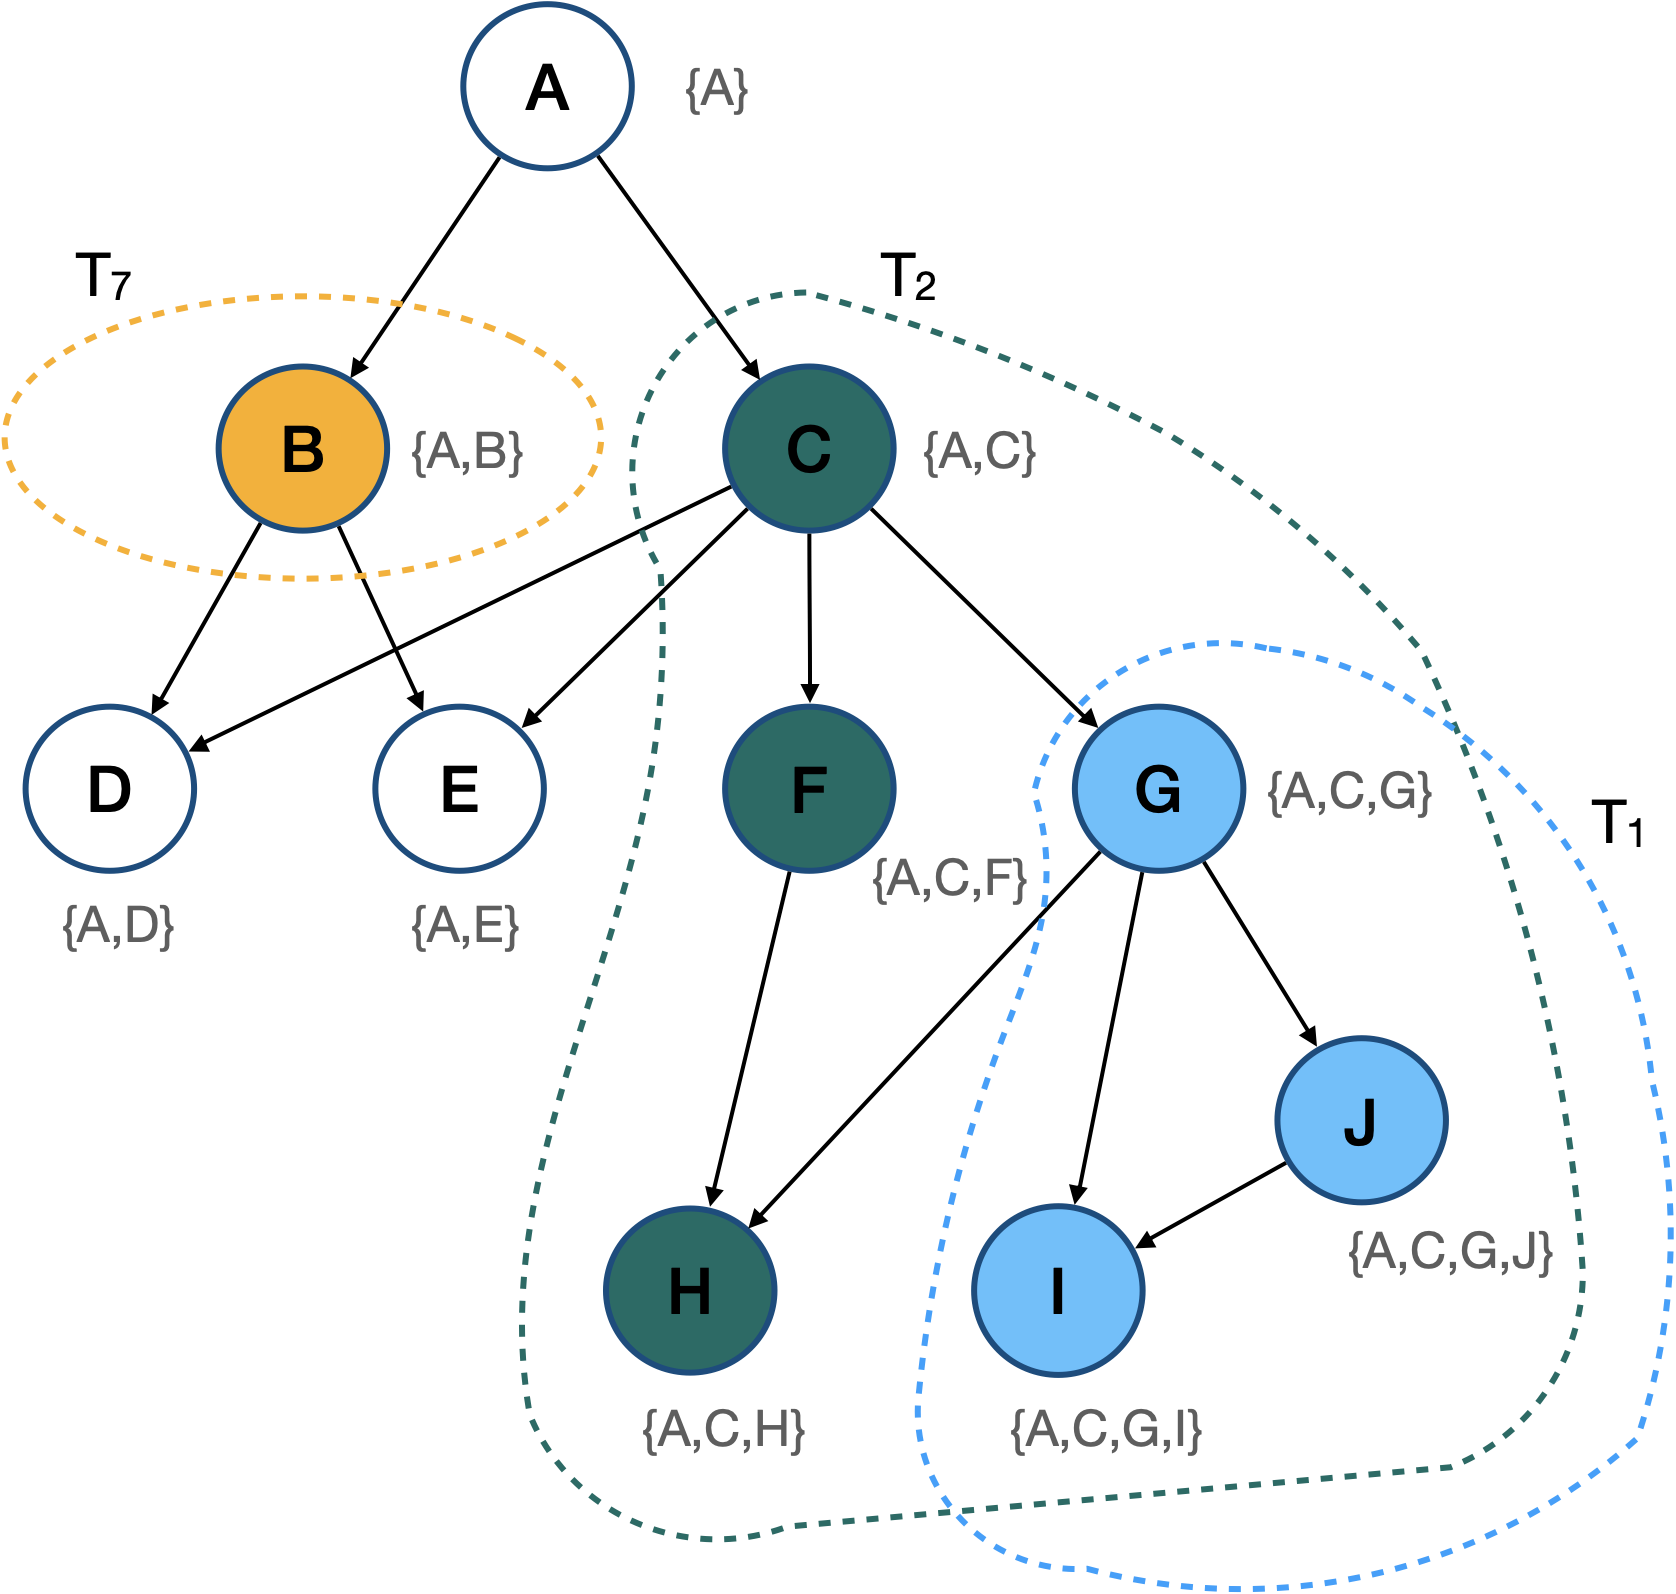
\includegraphics[width=.7\columnwidth]{figures/CALock_Lock_grains_inPool.png}
	\caption{Lock grains on the hierarchy for the locks requested by the threads in the lock pool(Figure \ref{lockPool})}
	\label{fig:lockGrainsOnHierarchy}
\end{figure}

Figure \ref{fig:lockPool} shows the snapshot of a lock pool. Figure \ref{fig:lockGrainsOnHierarchy} shows the grains on a hierarchy for the locks requested by threads in Figure \ref{fig:lockPool}. This pool contains requests from three threads $T_1, T_2$ and $T_7$. Suppose, $T_7$ arrives first and is assigned sequence number 1. $T_1$ and $T_2$ arrive later and have sequence numbers 2 and 3 respectively. 

$T_1$, $T_2$ and $T_7$ iterate over the pool from left to right and check for conflicts. $T_1$ finds a conflicting request at index 1 but has priority in the conflict since its sequence number is lower. Beyond index 1, it has no conflict in the pool and proceeds to acquire a read lock on G.

$T_2$ finds a conflicting request at index 0 and has a higher sequence number than $T_1$. So, $T_2$ waits for $T_1$ to release its lock. $T_1$ and $T_2$ conflict because they have overlapping grains. $T_2$ is requesting a lock on C which overlaps with the grain locked by $T_1$. This is confirmed by checking if C is present in the label of G i.e. $C \in \{A, C, G\}$.

$T_7$ does not conflict with any request and acquires a lock on B.



While checking for conflicts, a thread blocks at each conflict it encounters if its sequence number is higher than the conflicting request. A higher sequence number indicates that the thread arrived later and should wait for the conflicting thread to release the lock. 
Once a thread has iterated over the lock pool until the end, it is guaranteed to either have no conflicts with any request or have priority over all conflicts because its sequence number would be the lowest. We discuss this more in Chapter \ref{chap:formalProperties}.

% When requesting a lock, a thread $T$ can be blocked for a maximum of $n$ turns where $n$ is the size of the lock pool.
% After at most $n$ blocks, the sequence number of $T$ will be the lowest among all requests in the lock pool. As such, it will be allowed to proceed since it will be the oldest request in the pool and should be served first according to the first come first served ordering. 
% This is to prevent starvation.



		

\begin{algorithm}
	\caption{Lock acquisition request in the lock pool}\label{lockFunction}
	\begin{algorithmic}[1]
		\State $GSeq: $ Global sequence number for lock requests
		\State $Mutex: $ Mutex used when adding requests to the lock pool
		\State $Condition:$ Atomic boolean value used by waiting threads when in conflict
		\Statex
		\Procedure{Lock}{$req$, $threadID$}
		\State \Call{Lock}{$Mutex$}
		\State $req.Seq \gets Gseq++$ \label{seqNoAllocation}
		\State $req.condition.$\Call{TestAndSet}{true} \label{waitTrue}
		\State $Pool[threadId] \gets req$ \label{addToPool}
		\State \Call{Unlock}{$Mutex$}
		\ForAll{ $lock \in Pool \setminus threadID$} \label{conflictCheck}
		\If{ $lock \neq NULL$ \label{conditionCheck} 
			\State $\land(req.\Call{HasRWConflict}{$lock$})$
			\State $\land  (lock.guardID \in req.label \lor  req.guardID \in lock.label)$
			\State $\land (req.Seq > lock.Seq)$ 
		}
		\State $thread.$\Call{BlockAndwait}{$lock.condition$}
		\EndIf
		
		\EndFor
		\State return $true$
		\EndProcedure
		\Statex
		\Procedure{Unlock}{$lock$}
		\State $lockPool.$\Call{Remove}{$lock$}
		\State $lock.condition.$\Call{Clear}{ }
		\State $lock.condition.$\Call{notify\_all}{ }
		\EndProcedure
	\end{algorithmic}
\end{algorithm}






\section{Metadata Maintenance: Structural modifications and relabelling}

In the earlier sections, we discussed data accesses. The scope of a data access is limited to vertices. As such, a data access requires locking only vertices. Now, we study structural modifications. Structural modifications change a graph's topology, such as adding or deleting vertices and edges. These modifications require careful handling to ensure consistency. In this section, we will explore the mechanisms for locking and relabelling in CALock when structural modifications occur.

The same CALock algorithm, shown in Figure \ref{lockFunction} can be utilized for dynamic graphs that change at runtime. 
In order to perform a structural modification, a thread acquires a write lock on the LGCA of the affected vertices or the LGA if only one vertex is involved in a structural modification. For example, when adding an edge between vertices $u$ and $v$, a thread acquires a write lock on the LGCA of $u$ and $v$. 

% The lock protocol for a structural modification involves the following steps:

% \begin{enumerate}
% 	\item \textbf{Lock grain identification}: Identifying the grain of the vertices being modified. This is done by finding the LGCA of the vertices.
% 	\item \textbf{Lock request creation}: A lock request is created with the identified grain and \emph{write} mode.
% 	\item \textbf{Lock conflict detection}: The thread checks for mode and grain conflicts with other lock requests in the pool.
% 	\item \textbf{Operation execution}:	If no conflicts are detected, the thread proceeds to perform the structural modification. Vertices/edges are added or deleted.
% 	\item \textbf{Grain Relabelling}: Due to a change in the topology, the labels of the vertices in the affected grain may need to be updated. This is done by recursively calling the \inline|BFLabel()| function on the children of the affected vertices.
% 	\item \textbf{Lock release}: After relabelling terminates, the thread releases the lock on the grain.
% \end{enumerate}

A structural modification also involves a relabelling step for the affected grain. However, unlike DomLock, MID and FlexiGran in which the relabelling happens under a global mutex, relabelling in CALock is done under the same lock that is acquired to perform the structural modification. 
Here, we explain the locking and relabelling mechanism for dynamic graphs.

\subsection{Vertex addition and deletion}
Adding a vertex to the graph does not change the observable topology because this new vertex is not connected to the graph, and hence it is also not reachable from the root. 
So, vertex addition does not require locking or relabelling of any kind. The vertex gets a default label that contains its ID. 

Deleting a vertex that does not have any edges does not require synchronization either because such a vertex is not reachable from the root of the graph and also does not have children that might be affected.

\begin{figure}[h]
	\centering
	\captionsetup{justification=centering}
	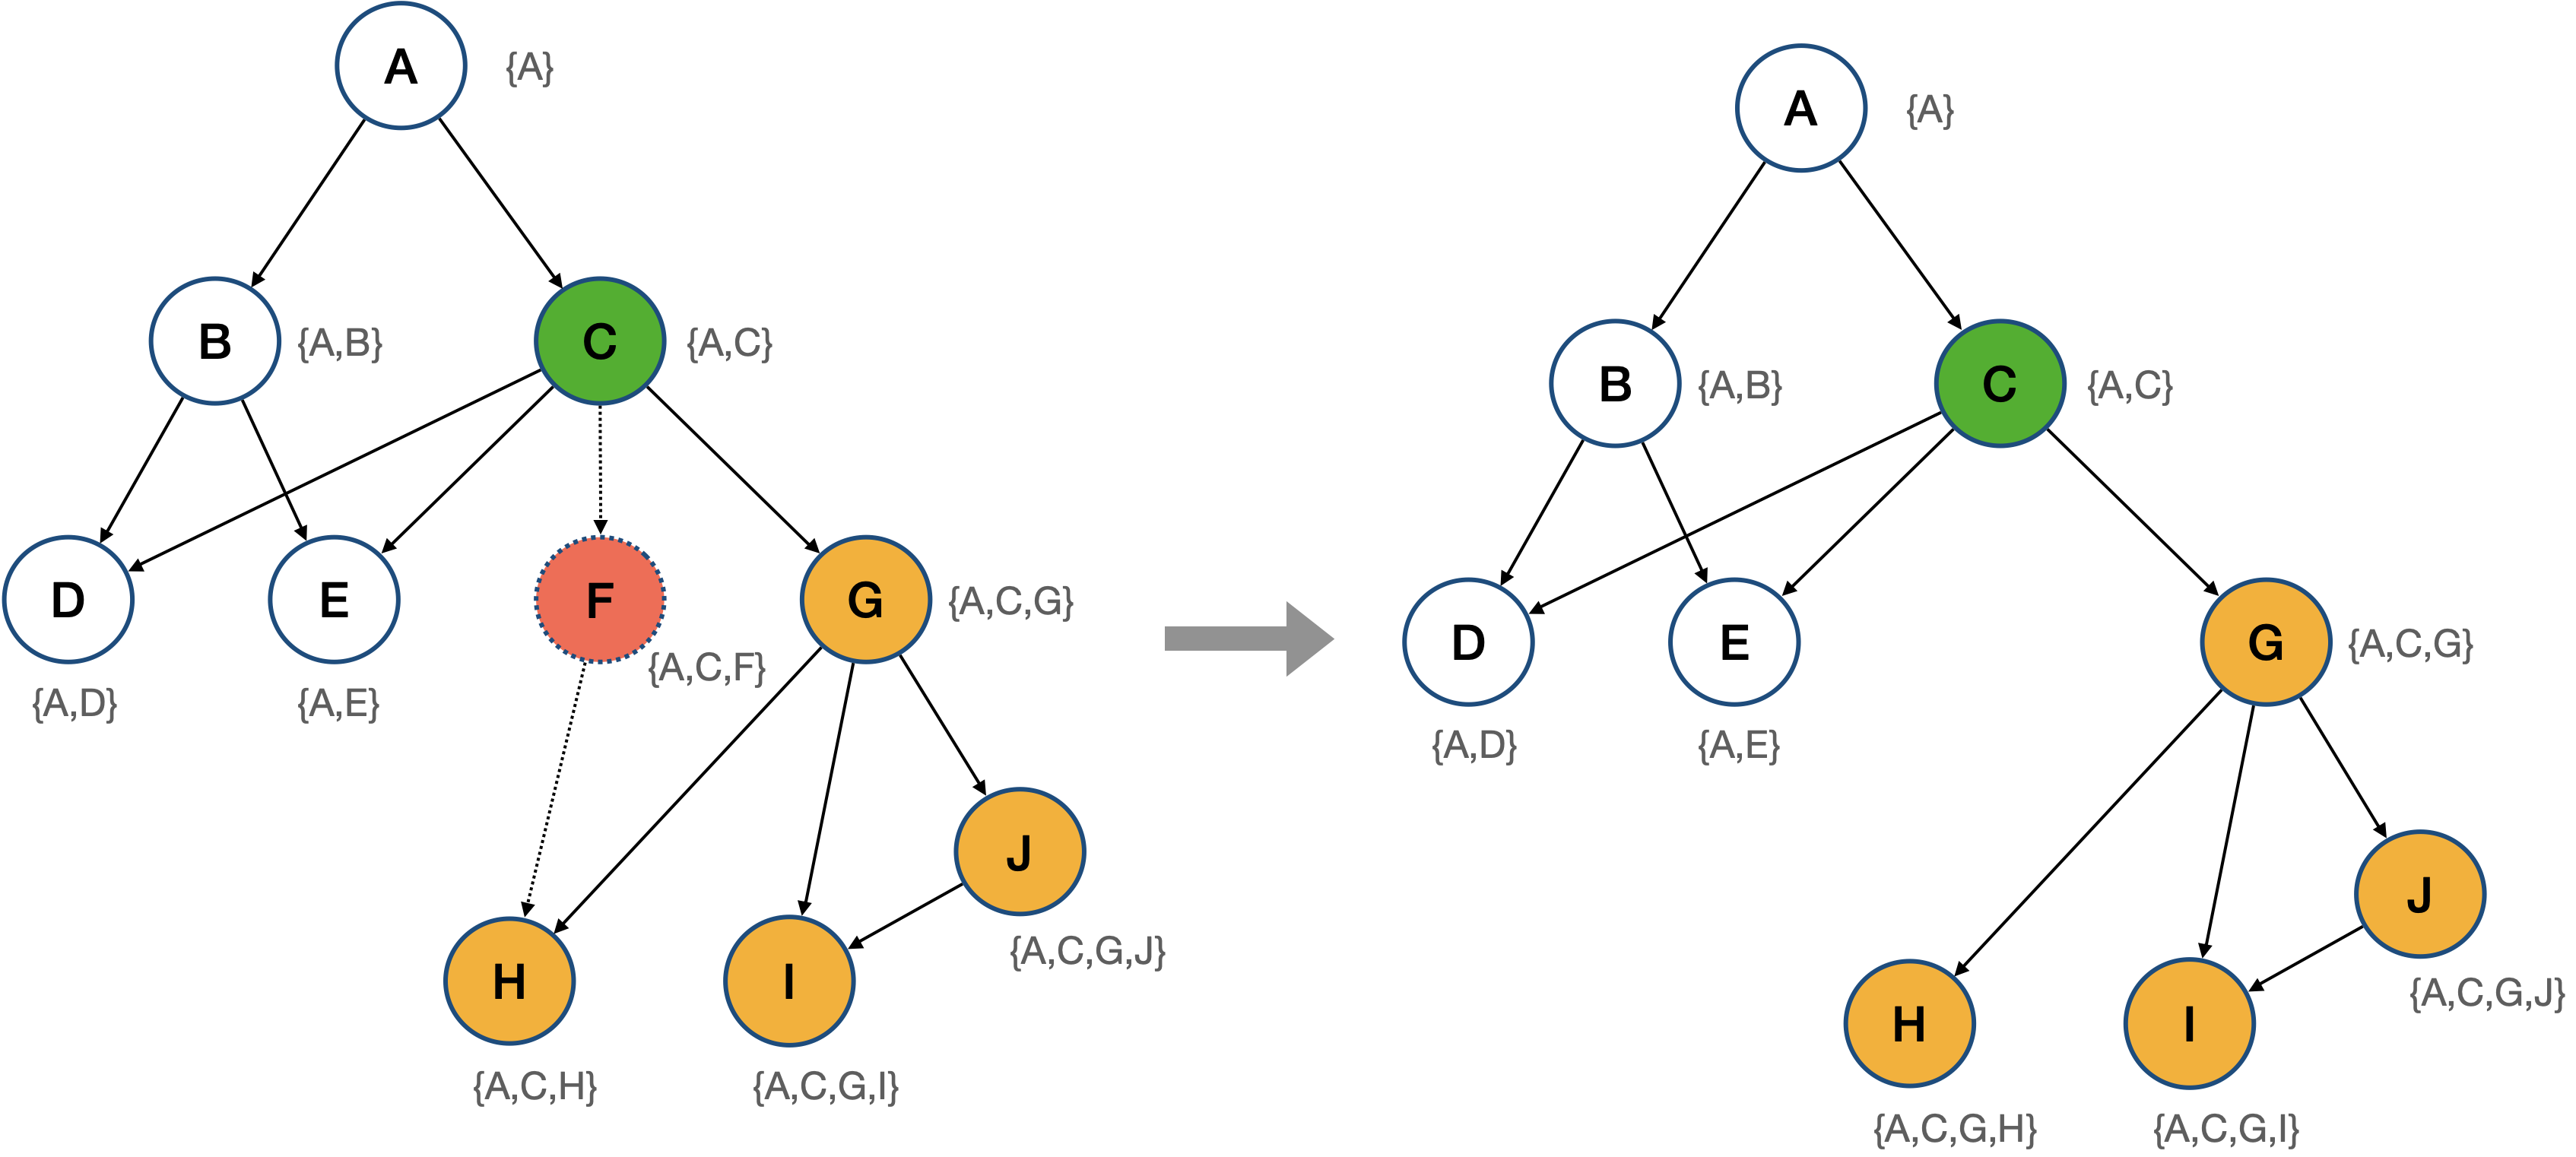
\includegraphics[width=\columnwidth]{figures/CALock_to_delete_vertex.png}
	\caption{In CALock, Deleting vertex H requires a lock on C}
	\label{fig:calockdelete}
\end{figure}

To delete a vertex that is reachable from the root, i.e., connected to the graph, a write lock is acquired on the LGA of the vertex that is to be deleted. 

The LGA can be computed by taking the second-last element in the label of the vertex to be deleted. The LGA guards the grain containing this vertex
Once the lock is acquired, the vertex is first disconnected from the graph by deleting all its edges and then deleted. Figure \ref{fig:calockdelete} shows an example where vertex F is deleted. To delete F, a lock is acquired on C which is the LGA of F.

After a vertex is deleted, relabelling might be necessary if the deleted vertex's descendants are still connected to the graph, since the set of their ancestors has changed. Relabelling is done by recursively calling the function \inline|BFLabel()| in Algorithm \ref{labelAssignment} on the children of the deleted vertex. 

In Figure \ref{fig:calockdelete}, F has one child, H. So, the label of H is recomputed. After F is deleted, H has only one parent, G. So, the label of H is recomputed as $\{A, C, G, H\}$.



\subsection{Edge addition and deletion}
Adding and deleting an edge changes the topology of a graph and also the paths to the vertices. 
Both operations are performed under a write (exclusive) lock. 

In order to add an edge between a source vertex $u$ and a target vertex $v$, a write lock is acquired on the LGCA of $u$ and $v$. This LGCA is computed by computing the set intersection of the labels of $u$ and $v$ i.e. $L_u \cap L_v$. The last vertex in this intersection is the LGCA of $u$ and $v$ and needs to be write locked to isolate the grain containing both $u$ and $v$.

\begin{figure}[h]
	\centering
	\captionsetup{justification=centering}
	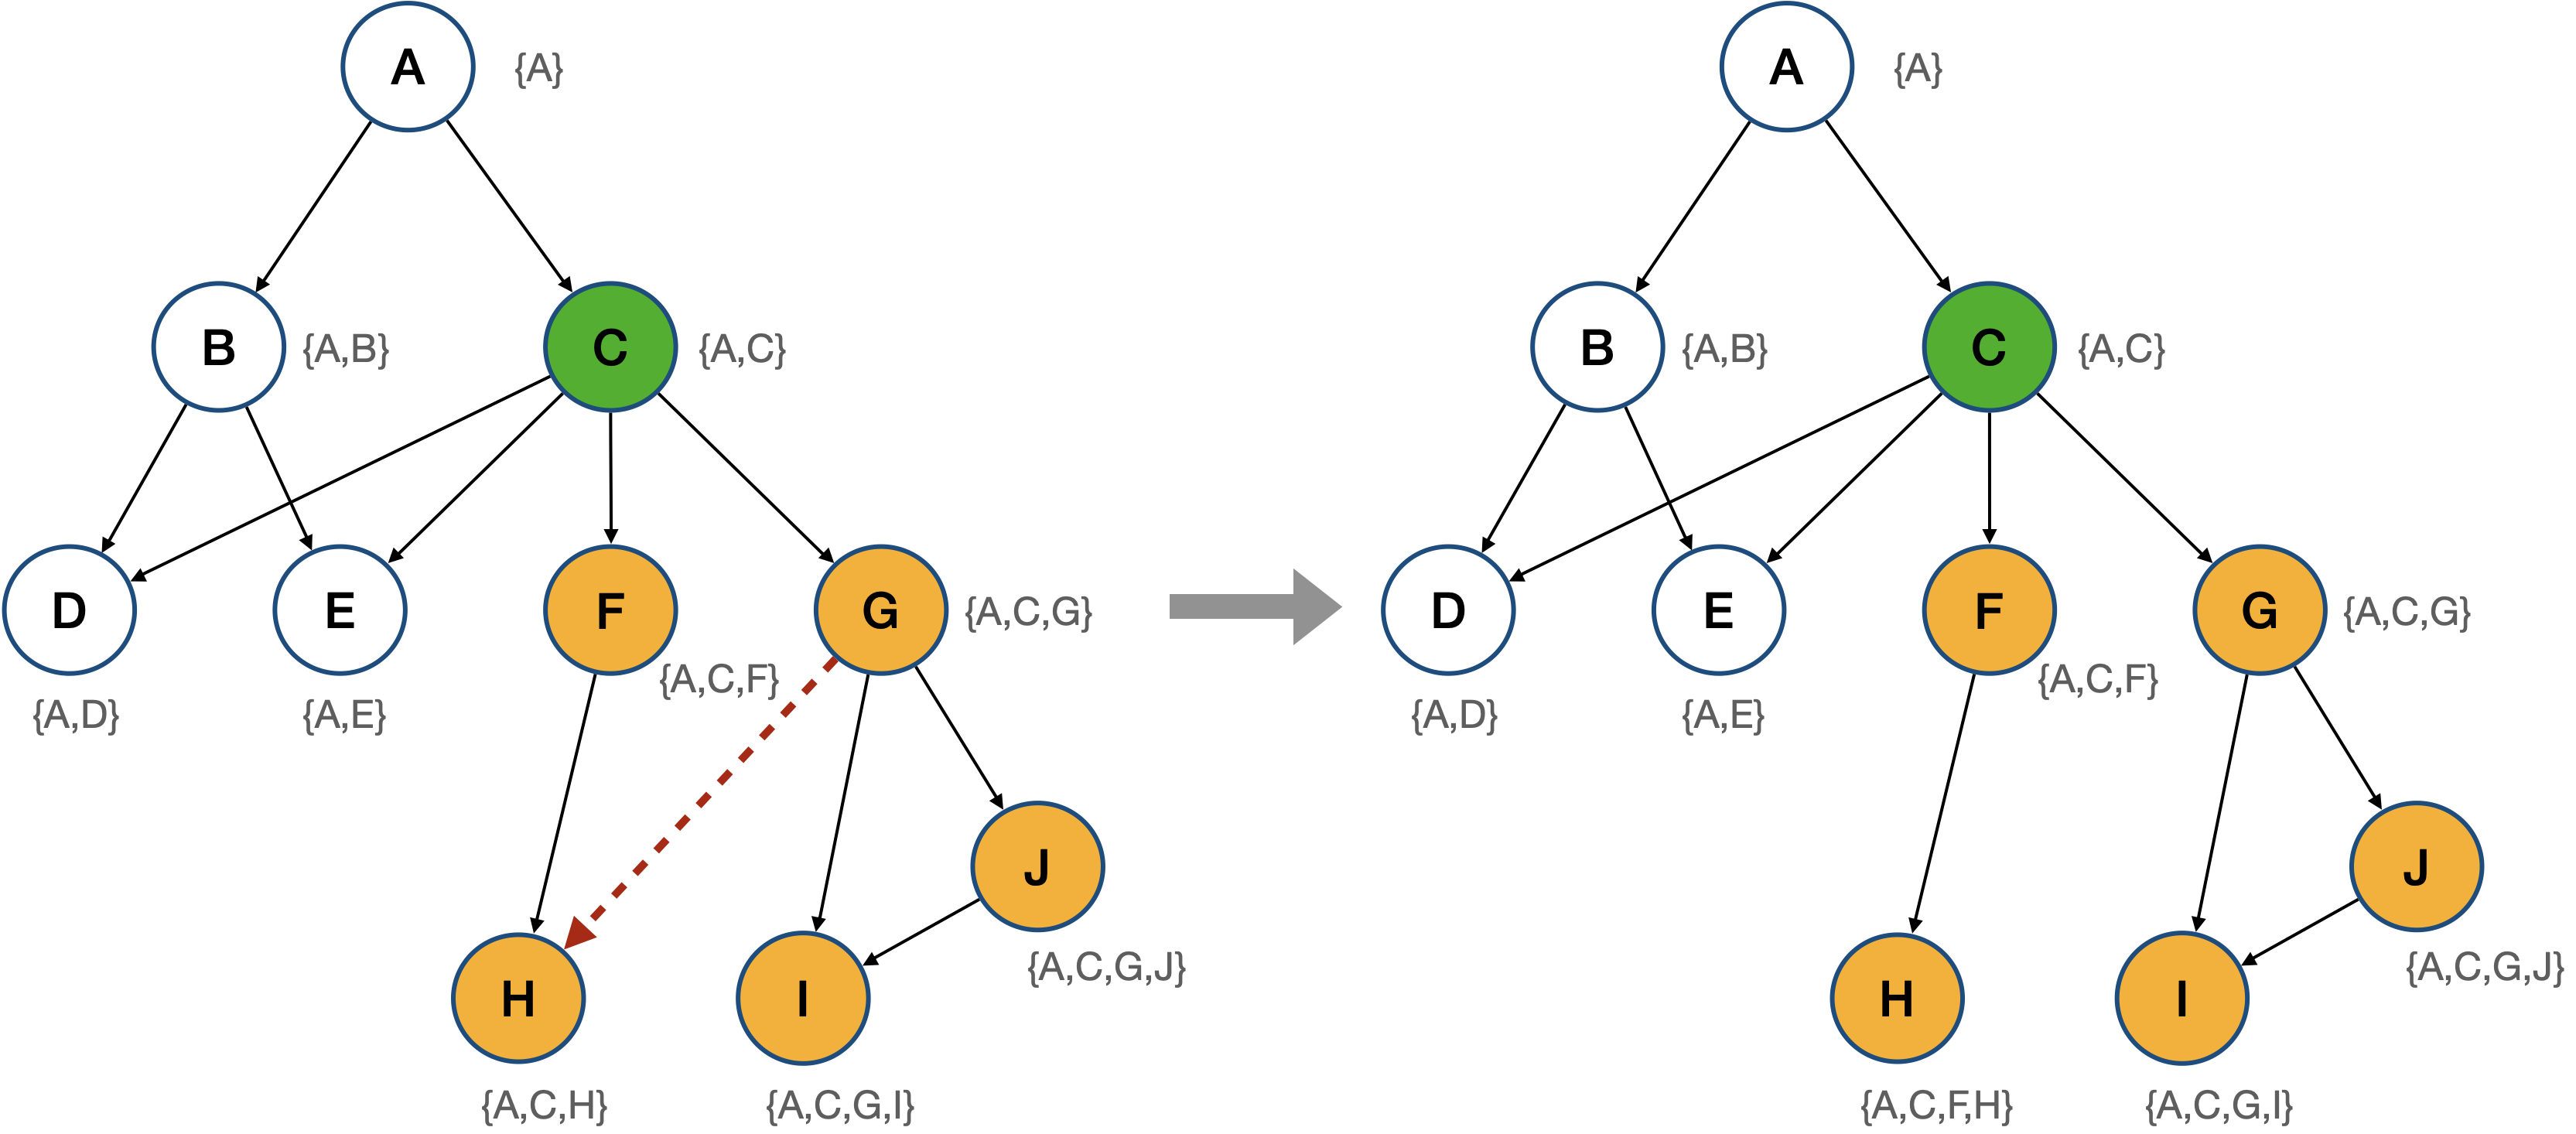
\includegraphics[width=\columnwidth]{figures/CALock_Delete_Edge.png}
	\caption{Deleting the edge between G and H requires a lock on C and relabelling of H}
	\label{fig:calockedgedeletion}
\end{figure}

Once a write lock is acquired, the operation can be performed. Adding or deleting an edge between two vertices changes the ancestors of the target vertex, so, relabelling is initiated at the target of the affected edge using \inline|BFLabel()| function. Figure \ref{fig:calockedgedeletion} shows an example where an edge is deleted between G and H. Prior to deleting, a lock is acquired on C which is the LGCA of G and H. After the edge is deleted, the target of the deleted edge, H, is relabelled. H has only one parent, F. So, the label of H is recomputed as $\{A, C, F, H\}$.

When a vertex has only one incoming edge, deleting that edge disconnects it from the graph. 
In this case, relabelling can be omitted because the target vertex $v$ has no parents and is also not reachable from the root of the graph. 


% \subsection{Relabeling}

% Relabeling involves the same steps as the initial labeling but is performed on the lock grain. This lock grain is a subgraph $G' = (V', E')$ of the graph $G = (V, E)$ such that
% \begin{itemize}
% 	\item $V' \subseteq V$ and $v' = \lvert V' \rvert$
% 	\item $E' \subseteq E \land ((v_1, v_2) \in E' \rightarrow v_1, v_2 \in V')$ and $e' = \lvert E' \rvert$
% \end{itemize}

% In most cases, the complexity of relabeling is proportional to the size of the grain i.e. $\theta(v'+ \frac{v'}{d_{avg}})$.
% In the best case, only a single vertex is locked. So the complexity of relabeling is $\Omega(1)$.
% In the worst case, $G' = G$ i.e. the whole graph is locked.
% This leads to a complexity of $O(2v)$



% \subsection{Conflict detection}
% Detecting lock conflicts involves iterating over a list that contains, at each index, the information of the lock grain.
% The complexity of iterating over the list is $O(n)$ where $n$ is the maximum number of threads.
